% !TEX program = lualatex
% Source: ../../2025/week7/week7.pdf (40 slides) and week7.ipynb.
\documentclass[12pt,aspectratio=43]{beamer}
% Shared Beamer design. Load after \documentclass using \input.
% Engine: LuaLaTeX. Fonts: UD Digi Kyokasho N (regular/bold), Arial.
\usepackage{luatexja-fontspec}
\setmainjfont[BoldFont={UD Digi Kyokasho N Bold}]{UD Digi Kyokasho N}
\setsansjfont[BoldFont={UD Digi Kyokasho N Bold}]{UD Digi Kyokasho N}
\setmonojfont[BoldFont={UD Digi Kyokasho N Bold}]{UD Digi Kyokasho N}
% Liberation Sans keeps the layout usable on systems without Arial.
\IfFontExistsTF{Arial}{
  \setmainfont{Arial}
  \setsansfont{Arial}
  \setmonofont{Arial}
}{
  \setmainfont{Liberation Sans}
  \setsansfont{Liberation Sans}
  \setmonofont{Liberation Sans}
}
\renewcommand{\kanjifamilydefault}{\gtdefault}

% Typeset mathematics with a dedicated TeX math font, independent of Arial.
\usefonttheme{professionalfonts}
\usepackage[mathrm=sym]{unicode-math}
\setmathfont{Latin Modern Math}
\setoperatorfont{\symup}

\definecolor{courseblue}{HTML}{4472C4}
\definecolor{ruleblue}{HTML}{8FAADC}
\setbeamercolor{normal text}{fg=black,bg=white}
\setbeamercolor{structure}{fg=courseblue}
\setbeamercolor{frametitle}{fg=black,bg=white}
\setbeamercolor{title banner}{fg=white,bg=courseblue}
\setbeamerfont{frametitle}{size=\fontsize{18}{22}\selectfont,series=\mdseries}
\setbeamerfont{quote}{shape=\upshape}
\setbeamersize{text margin left=9mm,text margin right=9mm}
\setbeamertemplate{navigation symbols}{}
\setbeamercolor{page number}{fg=gray,bg=white}
\setbeamertemplate{footline}{%
  \begin{beamercolorbox}[wd=\paperwidth,ht=2.5mm,dp=1.5mm]{page number}
    \hfill{\fontsize{8}{9}\selectfont
      \ifnum\value{framenumber}>0
        \insertframenumber\,/\,\inserttotalframenumber
      \fi}\hspace*{3mm}
  \end{beamercolorbox}}
\setbeamertemplate{headline}{%
  \hfill\textcolor{gray}{\fontsize{6}{7}\selectfont
    \hypersetup{linkcolor=gray}% Keep Beamer's title links in the header color.
    \ifnum\value{framenumber}=0 \insertshortdate\enspace\fi
    \insertshorttitle\space\insertshortsubtitle}\hspace{2mm}\vspace{1.5mm}}
\setbeamertemplate{frametitle}{%
  \vspace{2mm}\centering\insertframetitle\par
  \vspace{-1mm}{\color{ruleblue}\rule{.44\paperwidth}{.5pt}}\par
  \vspace{2mm}}
\setbeamercolor{itemize item}{fg=courseblue}
\setbeamercolor{itemize subitem}{fg=black}
\setbeamercolor{itemize subsubitem}{fg=black}
\setbeamertemplate{itemize item}{\textbullet}
\setbeamertemplate{itemize subitem}{\textnormal{-}}
\setbeamertemplate{itemize subsubitem}{\textnormal{-}}
\setlength{\parskip}{.45em}
\hypersetup{colorlinks=true,urlcolor=courseblue}

% Use \titlepage inside a [t,noframenumbering] frame. The background extends
% 1 mm past both page edges to avoid hairline gaps in PDF viewers.
\setbeamertemplate{title page}{%
  \vspace{2mm}
  \begin{beamercolorbox}[wd=\paperwidth,ht=43mm,dp=13mm,colsep*=1mm,center]{title banner}
    {\fontsize{32}{40}\selectfont\inserttitle\par}
    \vspace{2mm}
    {\fontsize{20}{24}\selectfont\insertsubtitle\par}
  \end{beamercolorbox}
  \vspace{10mm}
  \hfill\insertauthor
}

\graphicspath{{figures/}}
\usepackage{listings}
\usepackage{upquote}
\IfFontExistsTF{Consolas}{\newfontfamily\codefont{Consolas}}{\newfontfamily\codefont{Liberation Mono}}
\definecolor{codevalue}{HTML}{7A3E9D}
\definecolor{codebuiltin}{HTML}{006DB0}
\definecolor{codestring}{HTML}{267348}
\newcommand{\code}[1]{{\codefont #1}}
\lstdefinestyle{python}{
  language=Python,
  basicstyle=\codefont\fontsize{12}{14}\selectfont,
  keywordstyle=\color{codebuiltin},
  keywordstyle=[2]\color{codebuiltin},
  morekeywords=[2]{print,range},
  stringstyle=\color{codestring},
  showstringspaces=false,
  columns=fullflexible,
  keepspaces=true,
  upquote=true,
  tabsize=4,
  breaklines=false,
  backgroundcolor=\color{black!4},
  frame=single,framerule=0pt,framesep=1.7mm,
  xleftmargin=1.7mm,xrightmargin=1.7mm,
  aboveskip=1mm,belowskip=0.5mm,
  literate=*{0}{{{\color{codevalue}0}}}1
    {1}{{{\color{codevalue}1}}}1 {2}{{{\color{codevalue}2}}}1
    {3}{{{\color{codevalue}3}}}1 {4}{{{\color{codevalue}4}}}1
    {5}{{{\color{codevalue}5}}}1 {6}{{{\color{codevalue}6}}}1
    {7}{{{\color{codevalue}7}}}1 {8}{{{\color{codevalue}8}}}1
    {9}{{{\color{codevalue}9}}}1
}
\lstset{style=python}
\setbeamercolor{lesson note}{fg=black,bg=courseblue!9}
\newenvironment{lessonbox}
  {\begin{beamercolorbox}[wd=\linewidth,sep=1.5mm]{lesson note}}
  {\end{beamercolorbox}\par}

\title{計算物理学B}
\subtitle{第七回：数値積分}
\author{野垣 康介、藤本 悠輝}
\date{2026/12/1}
\hypersetup{pdftitle={計算物理学B 第七回：数値積分},pdfauthor={野垣 康介、藤本 悠輝}}

\begin{document}

\begin{frame}[t,noframenumbering]
  \titlepage
\end{frame}

\begin{frame}{講義予定}
  \setlength{\parskip}{0pt}
  2026年度 第2学期（火曜3限）
  \par\vspace{2mm}
  \begingroup\centering
    \renewcommand{\arraystretch}{1.05}
    \begin{tabular}{@{}l@{\hspace{2mm}}l@{\hspace{4mm}}l@{\hspace{2mm}}l@{}}
      10/6 & 四則演算 & 12/8 & モンテカルロ1 \\
      10/27 & 制御文（for, if） & 12/15 & モンテカルロ2 \\
      11/6（金） & 関数 & 12/22 & 微分方程式1 \\
      11/10 & 配列（NumPy） & 1/12 & 微分方程式2 \\
      11/17 & 可視化（matplotlib） & 1/19 & 偏微分方程式1 \\
      11/24 & 数値微分 & 1/26 & 偏微分方程式2 \\
      \textcolor{courseblue}{\textbf{12/1}} & \textcolor{courseblue}{\textbf{数値積分}} & 2/2 & 根の探索 \\
      \multicolumn{2}{c}{\small ～中間レポート～} & \multicolumn{2}{c}{\small ～期末レポート～}
    \end{tabular}\par
  \endgroup
  \vspace{2mm}
  {\small 10/20は出張で休講。11/6（金）は火曜授業の振替。\par}
  \vspace{1mm}
  {\fontsize{7}{8}\selectfont 日付：\href{https://www.niigata-u.ac.jp/wp-content/uploads/2025/08/schedule_2026.pdf}{令和8年度（2026）新潟大学授業暦}\par}
\end{frame}

\begin{frame}[t]{講義資料とノートブック}
  \begin{itemize}
    \setlength{\itemsep}{3mm}
    \item Google Colab：{\small\url{https://colab.research.google.com/?hl=ja}}
    \item 講義資料：{\small\url{https://github.com/nogaki/Computational_Physics_B}}
    \item 今週の教材：\code{2026/week7/}
    \item スライド：\code{slide.tex}、実習：\code{week7.ipynb}
  \end{itemize}
  \vspace{1mm}
  GitHubから開いたノートブックは、Colabの「ファイル」から\textbf{ドライブにコピーを保存}します。
  \vspace{2mm}
  \begin{lessonbox}
    課題・レポートの提出方法・期限は授業で案内します。
  \end{lessonbox}
\end{frame}

\begin{frame}[t]{今回の内容}
  \begin{itemize}
    \setlength{\itemsep}{3mm}
    \item 中点則・台形則・シンプソン則
    \item 適応求積とRomberg積分
    \item 不連続関数・端点特異点・無限区間
    \item Newton--Cotes公式とGauss--Legendre求積
  \end{itemize}
  \vfill
  \small 積分値を、関数の有限個の評価値から近似します。
\end{frame}

\begin{frame}[t]{数値積分が必要なとき}
  \[
    I=\int_a^b f(x)\,dx
  \]
  \begin{itemize}
    \setlength{\itemsep}{3mm}
    \item 原始関数が知られていない、または解析積分が難しい。
    \item 実験・シミュレーションで、関数値が一部の点でしか得られない。
    \item 高次元積分で、格子点の計算量が大きくなる。
  \end{itemize}
  \vspace{2mm}
  \begin{lessonbox}
    ここでは、区間上の関数を有限個の点で評価して積分を近似します。
  \end{lessonbox}
\end{frame}

\begin{frame}[t]{中点則：1区間}
  区間$[a,b]$での積分を、中点での関数値を使う長方形で近似します。
  \[
    \int_a^b f(x)\,dx\approx(b-a)f\!\left(\frac{a+b}{2}\right)
  \]
  幅$h=b-a$の局所誤差は
  \[
    I-M=\frac{h^3}{24}f''(\xi),\qquad a<\xi<b.
  \]
  \small $f$が線形なら$f''=0$なので、中点則は厳密です。
\end{frame}

\begin{frame}[t]{中点則の例}
  \[
    \int_0^2 (2x+3)\,dx=10
  \]
  線形関数では、1区間だけでも中点の長方形の面積が積分値と一致します。
  \vspace{3mm}
  \begin{lessonbox}
    曲率のある関数では、区間を分割して誤差を小さくします。
  \end{lessonbox}
\end{frame}

\begin{frame}[t]{合成中点則}
  $[a,b]$を$N$等分し、幅$h=(b-a)/N$の各小区間に中点則を適用します。
  \[
    M_N=h\sum_{k=1}^{N} f\!\left(a+\left(k-\frac12\right)h\right)
  \]
  滑らかな関数では
  \[
    I-M_N=\frac{h^2}{24}\left[f'(b)-f'(a)\right]+O(h^4),
  \]
  したがって全体の誤差は$O(h^2)$です。
\end{frame}

\begin{frame}[t]{中点則の分割と誤差}
  \begin{center}
    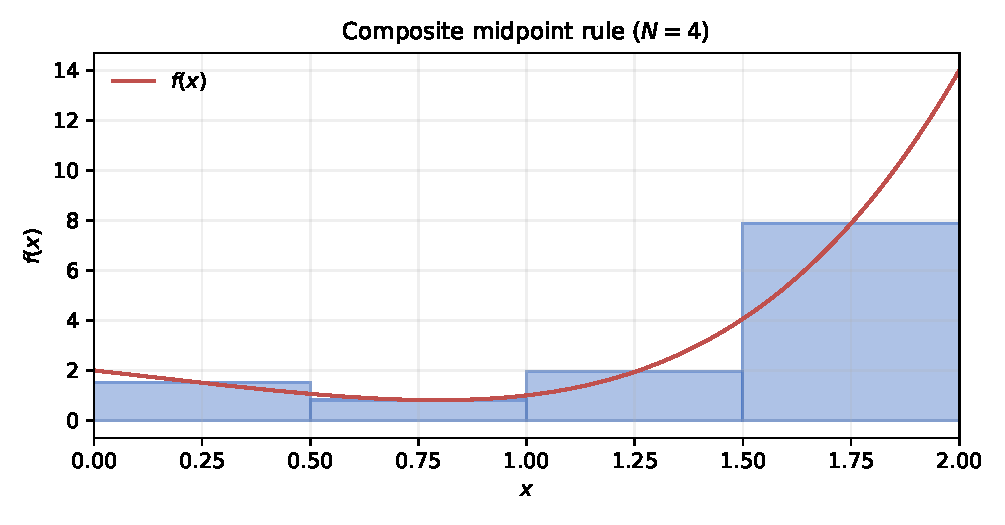
\includegraphics[width=.82\linewidth,height=43mm,keepaspectratio]{midpoint_rule.pdf}
  \end{center}
  \small 例：$f(x)=x^4-2x+2$を$[0,2]$で積分すると真値は$6.4$です。分割数$N$を増やすと、中点則の誤差はおよそ$N^{-2}$で減ります。
\end{frame}

\begin{frame}[t]{台形則：1区間}
  区間の端点を直線で結び、その下の台形の面積を使います。
  \[
    \int_a^b f(x)\,dx\approx (b-a)\frac{f(a)+f(b)}{2}
  \]
  局所誤差は
  \[
    I-T=-\frac{(b-a)^3}{12}f''(\xi),\qquad a<\xi<b.
  \]
  \small 台形則も線形関数に対して厳密です。凸関数では台形則は過大評価になります。
\end{frame}

\begin{frame}[t]{台形則の例}
  \[
    \int_0^2 (x^4-2x+2)\,dx=6.4
  \]
  端点を結ぶ線で各区間を近似します。
  \begin{center}
    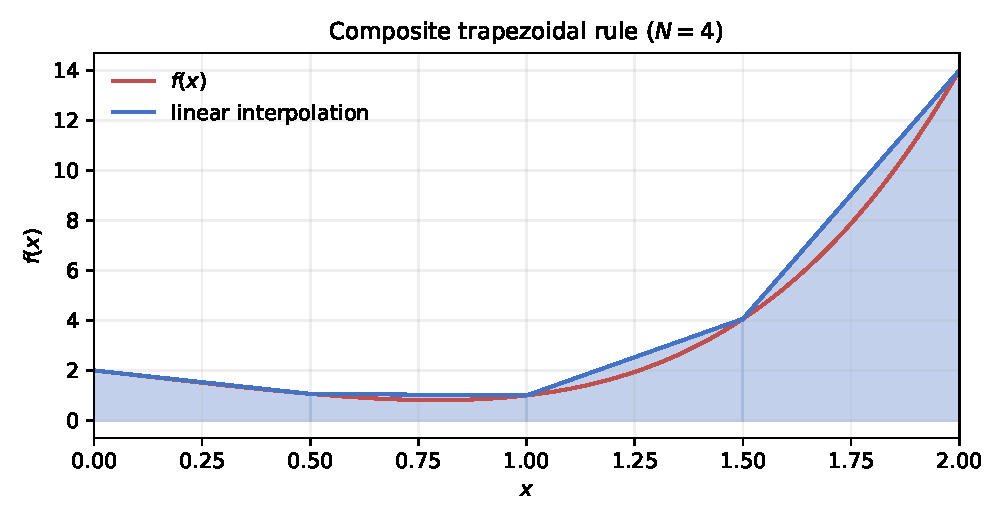
\includegraphics[width=.68\linewidth,height=28mm,keepaspectratio]{trapezoid_rule.pdf}
  \end{center}
  \small 凸関数では、台形則は過大評価になります。
\end{frame}

\begin{frame}[t]{合成台形則}
  $N$等分して各小区間の台形の面積を足します。
  \[
    T_N=h\left[\frac{f(x_0)+f(x_N)}{2}+\sum_{k=1}^{N-1}f(x_k)\right],\qquad x_k=a+kh.
  \]
  滑らかな関数の誤差は
  \[
    I-T_N=-\frac{h^2}{12}\left[f'(b)-f'(a)\right]+O(h^4),
  \]
  であり、全体で$O(h^2)$です。
\end{frame}

\begin{frame}[t]{中点則・台形則の比較}
  \begin{center}
    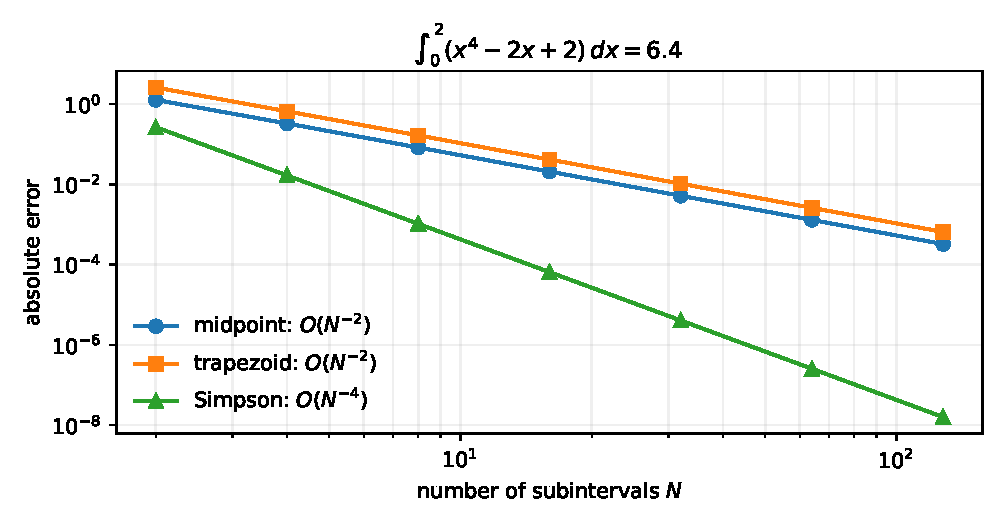
\includegraphics[width=.84\linewidth,height=43mm,keepaspectratio]{quadrature_convergence.pdf}
  \end{center}
  \small 同じ分割数では誤差の係数や符号が異なります。関数の形と必要な精度を見て方法を選びます。
\end{frame}

\begin{frame}[t]{精度を上げる2つの考え方}
  \begin{enumerate}
    \setlength{\itemsep}{4mm}
    \item 区間$[a,b]$を小区間に分け、低次の公式を合成する。
    \item 各小区間で高次の多項式を使い、近似の次数を上げる。
  \end{enumerate}
  \vspace{3mm}
  \begin{lessonbox}
    高次の公式は滑らかな関数で有効ですが、点の置き方と関数の滑らかさが重要です。
  \end{lessonbox}
\end{frame}

\begin{frame}[t]{シンプソン則：中点則と台形則の組合せ}
  同一区間の中点則$M$と台形則$T$は、$f''$に比例する主な誤差の符号と係数が異なります。
  \[
    S=\frac{2M+T}{3}
  \]
  と組み合わせると、$O(h^2)$の誤差項が相殺されます。
  \[
    \int_a^b f(x)\,dx\approx\frac{b-a}{6}\left[f(a)+4f\!\left(\frac{a+b}{2}\right)+f(b)\right]
  \]
\end{frame}

\begin{frame}[t]{シンプソン則の補間表示}
  区間の両端と中点の3点を通る2次多項式で$f(x)$を近似し、その多項式を積分します。
  \begin{center}
    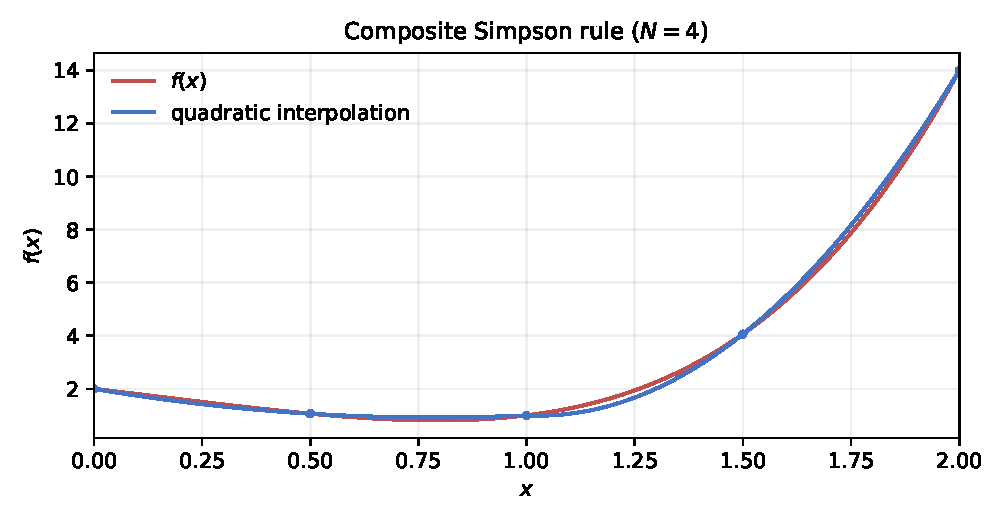
\includegraphics[width=.74\linewidth,height=38mm,keepaspectratio]{simpson_rule.pdf}
  \end{center}
\end{frame}

\begin{frame}[t]{合成シンプソン則}
  分割数$N$を偶数とし、幅$h=(b-a)/N$の2区間ごとに公式を適用します。
  \[
    S_N=\frac{h}{3}\left[f(x_0)+4\sum_{k=1}^{N/2}f(x_{2k-1})+2\sum_{k=1}^{N/2-1}f(x_{2k})+f(x_N)\right]
  \]
  滑らかな関数では誤差は$O(h^4)$です。
\end{frame}

\begin{frame}[t]{3つの合成公式の収束}
  \begin{center}
    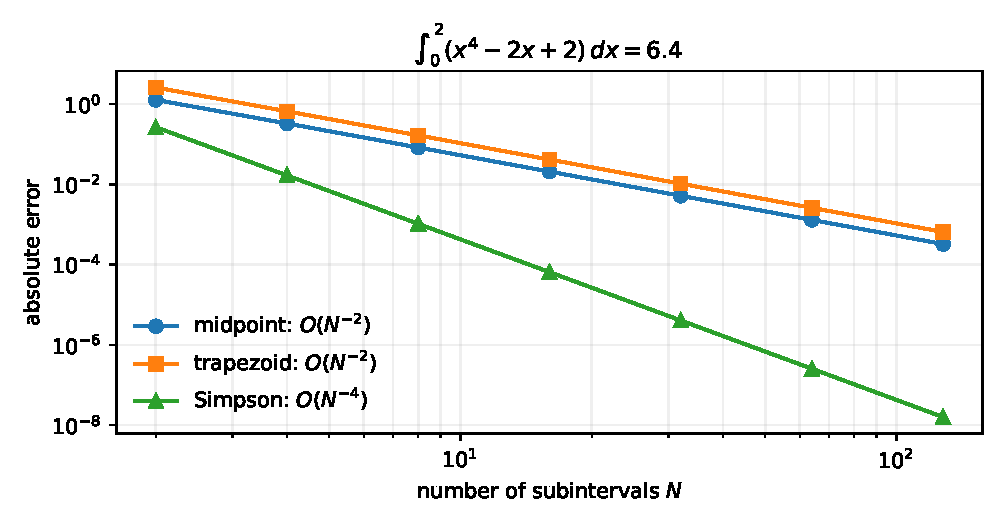
\includegraphics[width=.84\linewidth,height=43mm,keepaspectratio]{quadrature_convergence.pdf}
  \end{center}
  \small 中点則・台形則の誤差は$O(N^{-2})$、シンプソン則は$O(N^{-4})$です。$f(x)=x^4-2x+2$、$[0,2]$で比べています。
\end{frame}

\begin{frame}[t]{適応求積：誤差を見積もる}
  中点則や台形則の誤差が$O(h^2)$なら、分割数を2倍にしたとき誤差はおよそ4分の1です。
  \[
    I-I_{2N}\simeq\frac{I_{2N}-I_N}{3}
  \]
  分割を繰り返し、この誤差推定が許容値より小さくなったところで止めます。
  \small 推定が小さくても、関数に不連続や特異点があると誤差が過小評価される場合があります。
\end{frame}

\begin{frame}[t]{シンプソン則の適応求積}
  シンプソン則は$O(h^4)$なので、刻み幅を半分にすると誤差は約16分の1です。
  \[
    I-S_{2N}\simeq\frac{S_{2N}-S_N}{15}
  \]
  \begin{itemize}
    \item 誤差推定の絶対値が許容値を下回るまで分割します。
    \item 分割数は常に偶数にします。
    \item 収束判定と最大分割数の両方を用います。
  \end{itemize}
\end{frame}

\begin{frame}[t]{Romberg積分}
  台形則の値は、刻み幅$h$について
  \[
    T(h)=I+c_2h^2+c_4h^4+c_6h^6+\cdots
  \]
  と展開できます。
  \begin{itemize}
    \item $T(h)$と$T(h/2)$を組み合わせ、$h^2$項を消去します。
    \item さらに異なる刻み幅の値を組み合わせ、誤差項を順に消去します。
  \end{itemize}
  \small Richardson外挿を使う誤差改善法です。滑らかさを仮定するため、不連続関数では注意が必要です。
\end{frame}

\begin{frame}[t]{不連続な関数の積分}
  例として、$x=1$で跳びを持つ関数を考えます。
  \[
    f(x)=\begin{cases}
      3x^2+x+3,&x<1,\\
      2x^3-3x^2+x+3,&x\geq1.
    \end{cases}
  \]
  \[
    \int_0^2 f(x)\,dx=9.5
  \]
  \small 中点則・台形則でも積分できますが、分割点に不連続点が一致するよう区間を分けると扱いやすくなります。
\end{frame}

\begin{frame}[t]{不連続点で区間を分ける}
  \[
    I=\int_0^1 f_1(x)\,dx+\int_1^2 f_2(x)\,dx
  \]
  \begin{itemize}
    \item 各区間では関数が滑らかになり、誤差推定が働きやすくなります。
    \item 積分値の足し合わせで、全体の許容誤差を管理します。
    \item 数値積分では、既知の不連続位置を区間分割に反映します。
  \end{itemize}
  \vfill
  分割した積分の真値はそれぞれ$4.5$と$5.0$です。
\end{frame}

\begin{frame}[t]{端点に特異点がある積分}
  \[
    \int_0^1\frac{dx}{\sqrt{x}}=2
  \]
  被積分関数は$x=0$で発散しますが、積分値は有限です。
  \begin{itemize}
    \item 台形則など端点値を使う公式は、そのままでは評価できません。
    \item 中点則は端点を評価しませんが、特異性が残ると収束が遅い場合があります。
    \item 変数変換で特異性を取り除く方法があります。
  \end{itemize}
\end{frame}

\begin{frame}[t]{変数変換で特異性を取り除く}
  $x=t^2$と置くと、$dx=2t\,dt$です。
  \[
    \int_0^1\frac{dx}{\sqrt{x}}=\int_0^1\frac{2t}{\sqrt{t^2}}\,dt=\int_0^1 2\,dt=2
  \]
  \begin{lessonbox}
    変換後の関数が端点で有限になり、数値積分しやすくなります。
  \end{lessonbox}
  \small 台形則の失敗と、端点を使わない中点則の計算を比べます。
\end{frame}

\begin{frame}[t]{無限区間の積分}
  \[
    \int_a^\infty f(x)\,dx
  \]
  \[
    x=a+\frac{t}{1-t},\qquad dx=\frac{dt}{(1-t)^2}
  \]
  とすれば、半無限区間は$0\leq t<1$に移ります。
  \[
    \int_a^\infty f(x)\,dx=\int_0^1 f\!\left(a+\frac{t}{1-t}\right)\frac{dt}{(1-t)^2}
  \]
\end{frame}

\begin{frame}[t]{無限区間の例}
  \[
    \int_0^\infty e^{-x}\,dx=1
  \]
  変数変換後は
  \[
    \int_0^1 \frac{\exp\!\left(-\frac{t}{1-t}\right)}{(1-t)^2}\,dt.
  \]
  \begin{itemize}
    \item $t=1$は元の無限遠点に対応します。
    \item 端点での極限を確かめてから、数値公式に渡します。
  \end{itemize}
\end{frame}

\begin{frame}[t]{両側に無限区間がある積分}
  \[
    x=\frac{t}{1-t^2},\qquad dx=\frac{1+t^2}{(1-t^2)^2}\,dt
  \]
  とすると、$-\infty<x<\infty$は$-1<t<1$に移ります。
  \[
    \int_{-\infty}^{\infty}f(x)\,dx=\int_{-1}^1 f\!\left(\frac{t}{1-t^2}\right)\frac{1+t^2}{(1-t^2)^2}\,dt
  \]
  例：$\int_{-\infty}^{\infty}e^{-x^2}\,dx=\sqrt{\pi}$。
\end{frame}

\begin{frame}[t]{中点・台形・シンプソン則のまとめ}
  \small
  \begingroup\centering
    \renewcommand{\arraystretch}{1.6}
    \begin{tabular}{lll}
      方法 & 点と重み & 誤差（滑らかな関数） \\
      中点則 & 中点を使う & $O(h^2)$ \\
      台形則 & 端点を使う & $O(h^2)$ \\
      シンプソン則 & 端点と中点を使う & $O(h^4)$
    \end{tabular}\par
  \endgroup
  \vspace{3mm}
  求積公式は一般に
  \[
    \int_a^b f(x)\,dx\approx\sum_k w_k f(x_k)
  \]
  と書けます。$x_k$は積分点、$w_k$は重みです。
\end{frame}

\begin{frame}[t]{補間から高次の求積公式へ}
  $N+1$個の異なる点$(x_j,f(x_j))$を通る次数$N$以下の多項式を作ります。
  \[
    p_N(x)=\sum_{j=0}^{N}f(x_j)L_j(x)
  \]
  \[
    L_j(x)=\prod_{k\ne j}\frac{x-x_k}{x_j-x_k}
  \]
  これを積分すると
  \[
    \int_a^b f(x)\,dx\approx\sum_{j=0}^{N}w_jf(x_j),\qquad w_j=\int_a^b L_j(x)\,dx.
  \]
\end{frame}

\begin{frame}[t]{Lagrange補間多項式}
  基底多項式は補間点で$L_j(x_k)=\delta_{jk}$を満たし、各点で$p_N(x_j)=f(x_j)$となります。
  \begin{center}
    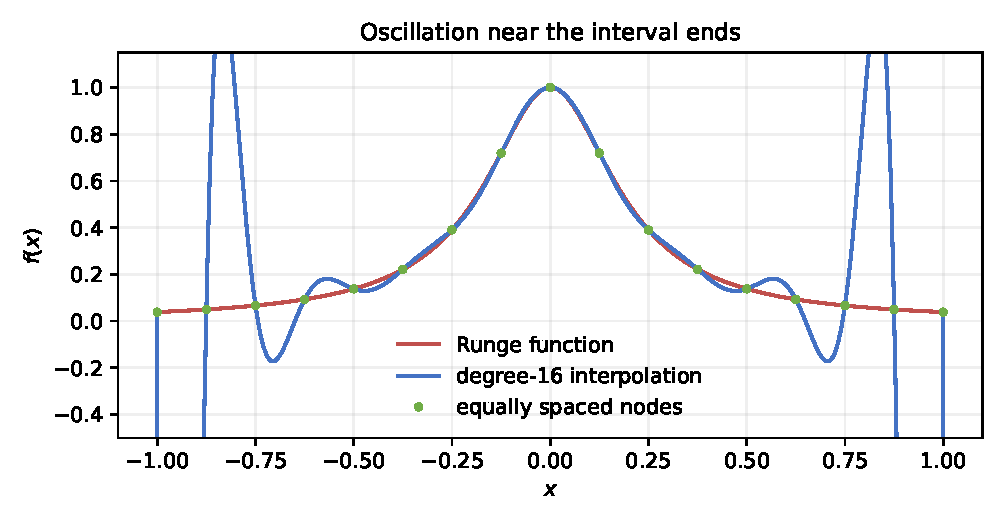
\includegraphics[width=.68\linewidth,height=34mm,keepaspectratio]{runge_interpolation.pdf}
  \end{center}
  \small 補間点を通ることと、区間全体で良く近似できることは別です。
\end{frame}

\begin{frame}[t]{Newton--Cotes求積法}
  Newton--Cotes公式では積分点を等間隔に取ります。
  \begin{itemize}
    \item 閉じた公式：端点を含む。$N=1$は台形則、$N=2$はシンプソン則。
    \item 開いた公式：端点を含まない。中点則もその一例です。
  \end{itemize}
  \vspace{2mm}
  \begin{lessonbox}
    点数を増やせば常に良くなるとは限りません。高次の等間隔補間はRunge現象を起こしえます。
  \end{lessonbox}
\end{frame}

\begin{frame}[t]{Runge現象と数値積分}
  Runge関数$f(x)=1/(1+25x^2)$を等間隔点で高次補間すると、区間端で振動が大きくなります。
  \begin{center}
    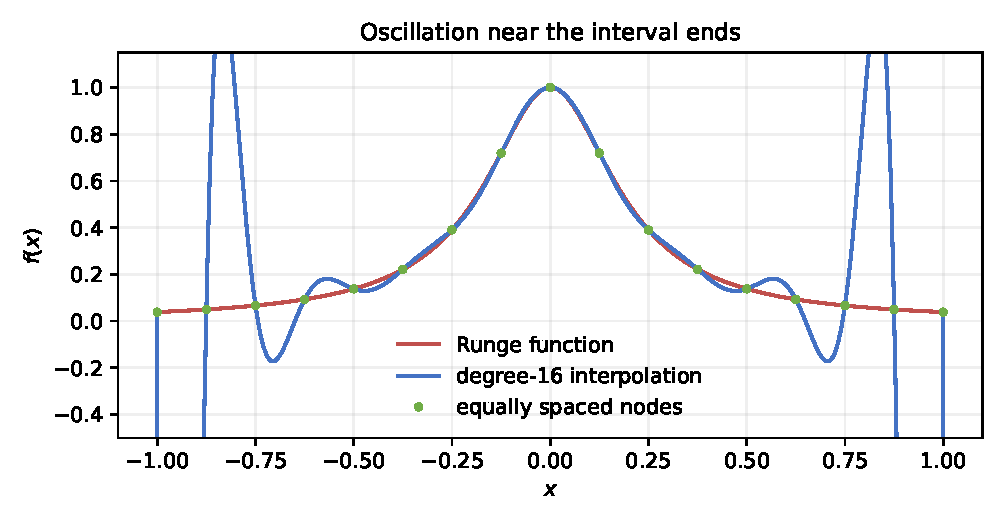
\includegraphics[width=.72\linewidth,height=31mm,keepaspectratio]{runge_interpolation.pdf}
  \end{center}
  \small 補間の振動は、積分値や誤差評価にも影響します。
\end{frame}

\begin{frame}[t]{Gauss--Legendre求積法}
  $n$点Gauss--Legendre公式は、重みと積分点を選び、$2n-1$次以下の多項式を厳密に積分します。
  \[
    \int_{-1}^{1} f(x)\,dx\approx\sum_{k=1}^{n}w_k f(x_k)
  \]
  \begin{itemize}
    \item 積分点$x_k$は$n$次Legendre多項式$P_n(x)$の零点です。
    \item 積分点は等間隔ではありません。
    \item 区間$[a,b]$には線形変換して適用します。
  \end{itemize}
\end{frame}

\begin{frame}[t]{Gauss--Legendre公式の区間変換}
  $z_k$と$w_k$を$[-1,1]$上のGauss--Legendre点と重みとします。
  \[
    x_k=\frac{b-a}{2}z_k+\frac{a+b}{2}
  \]
  \[
    \int_a^b f(x)\,dx\approx\frac{b-a}{2}\sum_{k=1}^{n}w_k f(x_k)
  \]
  \begin{lessonbox}
    $n$点公式は、次数$2n-1$までの多項式を厳密に積分します。
  \end{lessonbox}
\end{frame}

\begin{frame}[t]{方法を選ぶ}
  \small
  \begingroup\centering
    \renewcommand{\arraystretch}{1.5}
    \begin{tabular}{p{.23\linewidth}p{.31\linewidth}p{.29\linewidth}}
      方法 & 向いている場合 & 注意点 \\
      中点・台形・シンプソン & 単純な区間積分 & 分割数で精度を調整 \\
      適応求積・Romberg & 滑らかな関数、誤差制御 & 不連続や特異点に注意 \\
      Gauss--Legendre & 滑らかな関数、高精度 & 積分点は等間隔でない \\
      モンテカルロ & 高次元積分 & 標本誤差を見積もる
    \end{tabular}\par
  \endgroup
  \vspace{2mm}
  関数の滑らかさや次元に応じて方法を選びます。
\end{frame}

\begin{frame}[t]{高次元積分と計算量}
  $d$次元で各軸を$n$分割すると、格子点は$n^d$個になります。総点数を$N=n^d$とすると、次数$p$の格子法は概ね
  \[
    \text{誤差}=O(N^{-p/d})
  \]
  です。
  \[
    \text{モンテカルロの標準誤差}=O(N^{-1/2})
  \]
  \small 低次元では格子法、高次元ではモンテカルロ法が有利になる場合があります。
\end{frame}

\begin{frame}[t]{実習：中点則とシンプソン則}
  \[
    \int_0^2 x^7\,dx=32
  \]
  \begin{itemize}
    \setlength{\itemsep}{3mm}
    \item 中点則とシンプソン則で積分値を計算します。
    \item $N=4,16,64$で誤差を比べます。
    \item 4点Gauss--Legendre公式でも同じ積分を確かめます。
  \end{itemize}
  \vfill
  課題・レポートの提出方法・期限は授業で案内します。
\end{frame}

\begin{frame}[t]{参考資料}
  \begin{itemize}
    \setlength{\itemsep}{4mm}
    \item 野本拓也・是常隆・有田亮太郎『実践計算物理学』共立出版
    \item 水島二郎・柳瀬眞一郎『理工学のための数値計算法』数理工学社
    \item 参考にした講義資料：\url{https://github.com/vlvovch/PHYS6350-ComputationalPhysics}
  \end{itemize}
\end{frame}

\begin{frame}[t]{まとめ}
  \begin{itemize}
    \setlength{\itemsep}{3mm}
    \item 中点則・台形則は$O(h^2)$、シンプソン則は$O(h^4)$です。
    \item 適応求積は、分割ごとの計算値の差から誤差を推定します。
    \item 不連続点や特異点、無限区間は分割や変数変換で扱います。
    \item 高次公式では、等間隔点の補間振動に注意します。
  \end{itemize}
  \vfill
  次回：モンテカルロ法1
\end{frame}

\end{document}
